\documentclass[ignorenonframetext,]{beamer}
\setbeamertemplate{caption}[numbered]
\setbeamertemplate{caption label separator}{: }
\setbeamercolor{caption name}{fg=normal text.fg}
\beamertemplatenavigationsymbolsempty
\usepackage{lmodern}
\usepackage{amssymb,amsmath}
\usepackage{ifxetex,ifluatex}
\usepackage{fixltx2e} % provides \textsubscript
\ifnum 0\ifxetex 1\fi\ifluatex 1\fi=0 % if pdftex
  \usepackage[T1]{fontenc}
  \usepackage[utf8]{inputenc}
\else % if luatex or xelatex
  \ifxetex
    \usepackage{mathspec}
  \else
    \usepackage{fontspec}
  \fi
  \defaultfontfeatures{Ligatures=TeX,Scale=MatchLowercase}
\fi
% use upquote if available, for straight quotes in verbatim environments
\IfFileExists{upquote.sty}{\usepackage{upquote}}{}
% use microtype if available
\IfFileExists{microtype.sty}{%
\usepackage{microtype}
\UseMicrotypeSet[protrusion]{basicmath} % disable protrusion for tt fonts
}{}
\newif\ifbibliography
\hypersetup{
            pdftitle={Scala},
            pdfauthor={Konrad Siek},
            pdfborder={0 0 0},
            breaklinks=true}
\urlstyle{same}  % don't use monospace font for urls
\usepackage{color}
\usepackage{fancyvrb}
\newcommand{\VerbBar}{|}
\newcommand{\VERB}{\Verb[commandchars=\\\{\}]}
\DefineVerbatimEnvironment{Highlighting}{Verbatim}{commandchars=\\\{\}}
% Add ',fontsize=\small' for more characters per line
\usepackage{framed}
\definecolor{shadecolor}{RGB}{248,248,248}
\newenvironment{Shaded}{\begin{snugshade}}{\end{snugshade}}
\newcommand{\KeywordTok}[1]{\textcolor[rgb]{0.13,0.29,0.53}{\textbf{#1}}}
\newcommand{\DataTypeTok}[1]{\textcolor[rgb]{0.13,0.29,0.53}{#1}}
\newcommand{\DecValTok}[1]{\textcolor[rgb]{0.00,0.00,0.81}{#1}}
\newcommand{\BaseNTok}[1]{\textcolor[rgb]{0.00,0.00,0.81}{#1}}
\newcommand{\FloatTok}[1]{\textcolor[rgb]{0.00,0.00,0.81}{#1}}
\newcommand{\ConstantTok}[1]{\textcolor[rgb]{0.00,0.00,0.00}{#1}}
\newcommand{\CharTok}[1]{\textcolor[rgb]{0.31,0.60,0.02}{#1}}
\newcommand{\SpecialCharTok}[1]{\textcolor[rgb]{0.00,0.00,0.00}{#1}}
\newcommand{\StringTok}[1]{\textcolor[rgb]{0.31,0.60,0.02}{#1}}
\newcommand{\VerbatimStringTok}[1]{\textcolor[rgb]{0.31,0.60,0.02}{#1}}
\newcommand{\SpecialStringTok}[1]{\textcolor[rgb]{0.31,0.60,0.02}{#1}}
\newcommand{\ImportTok}[1]{#1}
\newcommand{\CommentTok}[1]{\textcolor[rgb]{0.56,0.35,0.01}{\textit{#1}}}
\newcommand{\DocumentationTok}[1]{\textcolor[rgb]{0.56,0.35,0.01}{\textbf{\textit{#1}}}}
\newcommand{\AnnotationTok}[1]{\textcolor[rgb]{0.56,0.35,0.01}{\textbf{\textit{#1}}}}
\newcommand{\CommentVarTok}[1]{\textcolor[rgb]{0.56,0.35,0.01}{\textbf{\textit{#1}}}}
\newcommand{\OtherTok}[1]{\textcolor[rgb]{0.56,0.35,0.01}{#1}}
\newcommand{\FunctionTok}[1]{\textcolor[rgb]{0.00,0.00,0.00}{#1}}
\newcommand{\VariableTok}[1]{\textcolor[rgb]{0.00,0.00,0.00}{#1}}
\newcommand{\ControlFlowTok}[1]{\textcolor[rgb]{0.13,0.29,0.53}{\textbf{#1}}}
\newcommand{\OperatorTok}[1]{\textcolor[rgb]{0.81,0.36,0.00}{\textbf{#1}}}
\newcommand{\BuiltInTok}[1]{#1}
\newcommand{\ExtensionTok}[1]{#1}
\newcommand{\PreprocessorTok}[1]{\textcolor[rgb]{0.56,0.35,0.01}{\textit{#1}}}
\newcommand{\AttributeTok}[1]{\textcolor[rgb]{0.77,0.63,0.00}{#1}}
\newcommand{\RegionMarkerTok}[1]{#1}
\newcommand{\InformationTok}[1]{\textcolor[rgb]{0.56,0.35,0.01}{\textbf{\textit{#1}}}}
\newcommand{\WarningTok}[1]{\textcolor[rgb]{0.56,0.35,0.01}{\textbf{\textit{#1}}}}
\newcommand{\AlertTok}[1]{\textcolor[rgb]{0.94,0.16,0.16}{#1}}
\newcommand{\ErrorTok}[1]{\textcolor[rgb]{0.64,0.00,0.00}{\textbf{#1}}}
\newcommand{\NormalTok}[1]{#1}
\usepackage{graphicx,grffile}
\makeatletter
\def\maxwidth{\ifdim\Gin@nat@width>\linewidth\linewidth\else\Gin@nat@width\fi}
\def\maxheight{\ifdim\Gin@nat@height>\textheight0.8\textheight\else\Gin@nat@height\fi}
\makeatother
% Scale images if necessary, so that they will not overflow the page
% margins by default, and it is still possible to overwrite the defaults
% using explicit options in \includegraphics[width, height, ...]{}
\setkeys{Gin}{width=\maxwidth,height=\maxheight,keepaspectratio}

% Prevent slide breaks in the middle of a paragraph:
\widowpenalties 1 10000
\raggedbottom

\AtBeginPart{
  \let\insertpartnumber\relax
  \let\partname\relax
  \frame{\partpage}
}
\AtBeginSection{
  \ifbibliography
  \else
    \let\insertsectionnumber\relax
    \let\sectionname\relax
    \frame{\sectionpage}
  \fi
}
\AtBeginSubsection{
  \let\insertsubsectionnumber\relax
  \let\subsectionname\relax
  \frame{\subsectionpage}
}

\setlength{\parindent}{0pt}
\setlength{\parskip}{6pt plus 2pt minus 1pt}
\setlength{\emergencystretch}{3em}  % prevent overfull lines
\providecommand{\tightlist}{%
  \setlength{\itemsep}{0pt}\setlength{\parskip}{0pt}}
\setcounter{secnumdepth}{0}

\title{Scala}
\subtitle{An abrupt introduction}
\author{Konrad Siek}
\date{September, 2019}

\begin{document}
\frame{\titlepage}

\begin{frame}[fragile]

\begin{block}{Course information}

\textbf{BIE-OOP}\\
Object Oriented Programming

\textbf{Course website}: \url{https://courses.fit.cvut.cz/BI-OOP/}

\end{block}

\begin{block}{Contact information}

\textbf{Ing. Konrad Siek, PhD.}\\
Programming Research Lab\\
Faculty of Information Technology

\textbf{Office}: Thákurova 7, A-1252\\
\textbf{Email}:
\href{mailto:siekkonr@fit.cvut.cz}{\nolinkurl{siekkonr@fit.cvut.cz}}\\
\textbf{My website}: \url{https://kondziu.github.io/}

\textbf{Office hours}: Wednesdays 10:00-11:00

\begin{figure}
\centering
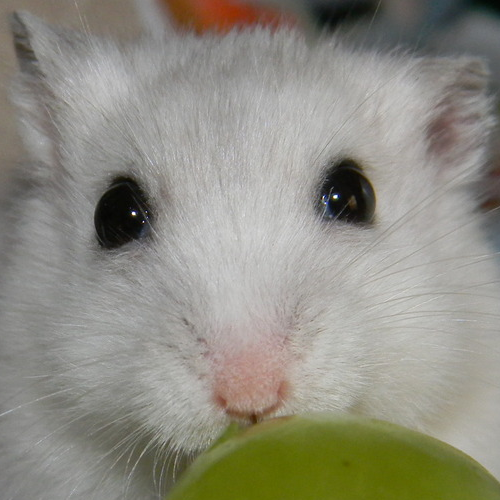
\includegraphics[height=2.08333in]{hamstur.png}
\caption{Real picture}
\end{figure}

\end{block}

\begin{block}{What is Scala?}

\begin{quote}
Scala combines \textbf{object-oriented} and \textbf{functional
programming} in one \textbf{concise}, \textbf{high-level} language.
Scala's \textbf{static types} help avoid bugs in complex applications,
and its \textbf{JVM} and \textbf{JavaScript} runtimes let you build
\textbf{high-performance} systems with easy access to huge
\textbf{ecosystems of libraries}.
\end{quote}

\href{https://www.scala-lang.org}{\textbf{scala-lang.org}}

\end{block}

\begin{block}{What is Scala?}

Scala is a modern \textbf{multi-paradigm programming language} designed
to express common programming patterns in a \textbf{concise},
\textbf{elegant}, and \textbf{type-safe way}. It smoothly integrates
features of \textbf{object-oriented} and \textbf{functional languages}.

\href{https://docs.scala-lang.org/tour/tour-of-scala.html}{\textbf{Tour
of Scala}}.

\end{block}

\begin{block}{What is Scala?}

2003 - A drunken \textbf{Martin Odersky} sees a Reese's Peanut Butter
Cup ad featuring somebody's peanut butter getting on somebody else's
chocolate and has an idea. He creates Scala, a language that
\textbf{unifies constructs} from both \textbf{object oriented} and
\textbf{functional languages}. This pisses off both groups and each
promptly declares jihad.

James Iry.
\href{http://james-iry.blogspot.com/2009/05/brief-incomplete-and-mostly-wrong.html}{\textbf{A
Brief, Incomplete, and Mostly Wrong History of Programming Languages}}.
2009.

\end{block}

\begin{block}{What is Scala?}

\begin{figure}
\centering
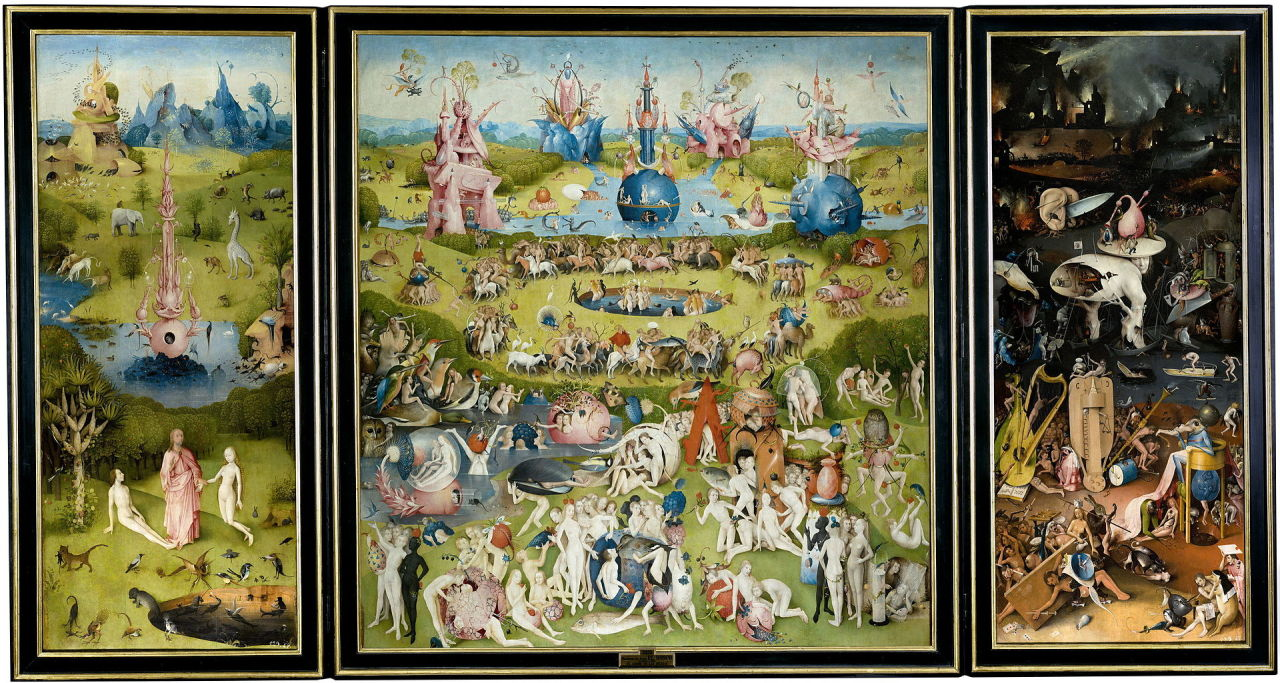
\includegraphics[width=5.20833in]{bosch.jpg}
\caption{A visual guide to the Scala language}
\end{figure}

Hieronymus Bosch.
\href{https://classicprogrammerpaintings.com/post/142321815809/hieronymus-bosch-a-visual-guide-to-the-scala}{\textbf{A
visual guide to the Scala language}}. Oil on oak panels, 1490-1510.

The left panel shows the \textbf{functional features}, the main one
describes the \textbf{type system}, and the right the \textbf{object
oriented parts}.

\end{block}

\begin{block}{Expressions}

\begin{Shaded}
\begin{Highlighting}[]
\DecValTok{2}\NormalTok{ + }\DecValTok{3}
\DecValTok{2}\NormalTok{ - }\DecValTok{3} 
\DecValTok{2}\NormalTok{ * }\DecValTok{3}
\DecValTok{2}\NormalTok{ / }\DecValTok{3}
\DecValTok{2}\NormalTok{ % }\DecValTok{3}

\DecValTok{2}\NormalTok{ ^ }\DecValTok{3}
\DecValTok{2}\NormalTok{ & }\DecValTok{3}
\DecValTok{2}\NormalTok{ | }\DecValTok{3}

\DecValTok{2}\NormalTok{ >> }\DecValTok{3}
\DecValTok{2}\NormalTok{ << }\DecValTok{3}
\end{Highlighting}
\end{Shaded}

\begin{Shaded}
\begin{Highlighting}[]
\StringTok{"ahoj"}
\StringTok{"ahoj"}\NormalTok{ + }\DecValTok{2}
\StringTok{"ahoj"}\NormalTok{ * }\DecValTok{2}

\StringTok{"ahoj"}\NormalTok{ + }\StringTok{" "}\NormalTok{ + }\StringTok{"světe!"}
\end{Highlighting}
\end{Shaded}

\begin{Shaded}
\begin{Highlighting}[]
\DecValTok{1}\NormalTok{ == }\DecValTok{2}
\DecValTok{1}\NormalTok{ >= }\DecValTok{2}
\DecValTok{1}\NormalTok{ <= }\DecValTok{2}
\end{Highlighting}
\end{Shaded}

\begin{Shaded}
\begin{Highlighting}[]
\StringTok{"a"}\NormalTok{ -> }\DecValTok{2}
\end{Highlighting}
\end{Shaded}

\end{block}

\begin{block}{Values}

\begin{Shaded}
\begin{Highlighting}[]
\KeywordTok{val}\NormalTok{ x = }\DecValTok{5}
\KeywordTok{val}\NormalTok{ s = }\StringTok{"spaceship"}
\KeywordTok{val}\NormalTok{ y : Int = }\DecValTok{0}
\end{Highlighting}
\end{Shaded}

\end{block}

\begin{block}{Variables}

\begin{Shaded}
\begin{Highlighting}[]
\KeywordTok{var}\NormalTok{ vx = }\DecValTok{5}
\KeywordTok{var}\NormalTok{ vs = }\StringTok{"spaceship"}
\KeywordTok{var}\NormalTok{ vy : Int = }\DecValTok{0}
\end{Highlighting}
\end{Shaded}

\begin{Shaded}
\begin{Highlighting}[]
\NormalTok{x = }\DecValTok{42}
\NormalTok{vx = }\DecValTok{42}
\end{Highlighting}
\end{Shaded}

\end{block}

\begin{block}{Default values}

\begin{Shaded}
\begin{Highlighting}[]
\KeywordTok{var}\NormalTok{ x : Int = _}
\KeywordTok{var}\NormalTok{ s : String = _}
\end{Highlighting}
\end{Shaded}

\end{block}

\begin{block}{Everything is an object}

\begin{Shaded}
\begin{Highlighting}[]
\FloatTok{5.}\FunctionTok{toString}\NormalTok{()}
\end{Highlighting}
\end{Shaded}

\end{block}

\begin{block}{Operators are methods}

\begin{Shaded}
\begin{Highlighting}[]
\KeywordTok{val}\NormalTok{ x, y = }\DecValTok{2}

\NormalTok{x + y}
\NormalTok{x.+(y)}
\end{Highlighting}
\end{Shaded}

\end{block}

\begin{block}{Infix notation}

\begin{Shaded}
\begin{Highlighting}[]
\KeywordTok{val}\NormalTok{ s = }\StringTok{"something something spaceship"}
\NormalTok{s.}\FunctionTok{split}\NormalTok{(}\StringTok{" "}\NormalTok{)}
\NormalTok{s }\FunctionTok{split}\NormalTok{(}\StringTok{" "}\NormalTok{)}
\NormalTok{s split }\StringTok{" "}
\end{Highlighting}
\end{Shaded}

Only use with \textbf{arity 1 pure functions}. Strongly encouraged if
the argument is a function.

(\href{http://docs.scala-lang.org/style/method-invocation.html}{Scala
style guide})

\end{block}

\begin{block}{Omitting parentheses}

\begin{Shaded}
\begin{Highlighting}[]
\KeywordTok{val}\NormalTok{ x = }\DecValTok{2}
\NormalTok{x.}\FunctionTok{toString}\NormalTok{()}
\NormalTok{x.}\FunctionTok{toString}
\NormalTok{x toString}
\end{Highlighting}
\end{Shaded}

Only use with \textbf{arity 0 pure functions}.

(\href{http://docs.scala-lang.org/style/method-invocation.html}{Scala
style guide})

\end{block}

\begin{block}{Unified types}

\begin{figure}
\centering
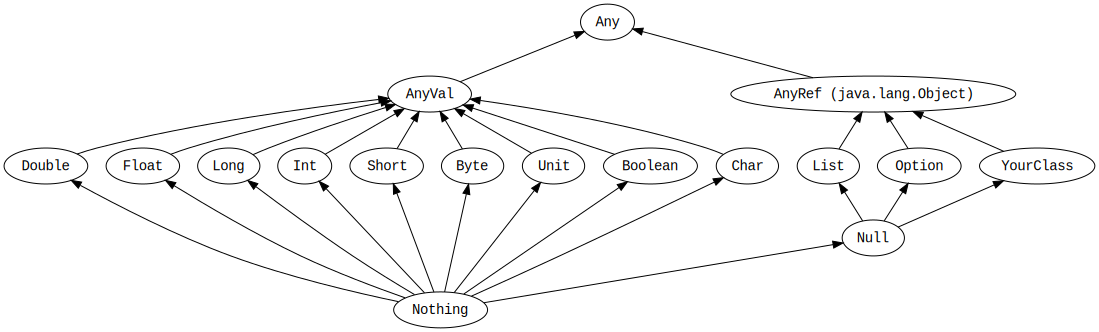
\includegraphics[width=8.33333in]{unified-types-diagram.svg}
\caption{Unified types}
\end{figure}

\end{block}

\begin{block}{Casting}

\begin{Shaded}
\begin{Highlighting}[]
\KeywordTok{val}\NormalTok{ i:Int = }\DecValTok{1}
\KeywordTok{val}\NormalTok{ d:Double = i}
\end{Highlighting}
\end{Shaded}

\begin{Shaded}
\begin{Highlighting}[]
\KeywordTok{val}\NormalTok{ d:Double = }\FloatTok{1.0}\NormalTok{d}
\KeywordTok{val}\NormalTok{ i:Int = d}
\end{Highlighting}
\end{Shaded}

\end{block}

\begin{block}{Casting order}

\begin{figure}
\centering
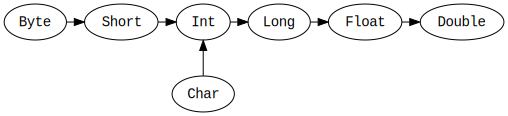
\includegraphics{type-casting-diagram.svg}
\caption{Type casting diagram}
\end{figure}

\end{block}

\begin{block}{Explicit casting}

\begin{Shaded}
\begin{Highlighting}[]
\FloatTok{0.}\NormalTok{asInstanceOf[Char]}
\FloatTok{1.}\NormalTok{asInstanceOf[Double]}
\FloatTok{2.}\NormalTok{asInstanceOf[Float]}
\CharTok{'a'}\NormalTok{.}\FunctionTok{asInstanceOf}\NormalTok{[Int]}
\end{Highlighting}
\end{Shaded}

\end{block}

\begin{block}{Tupples}

\begin{Shaded}
\begin{Highlighting}[]
\KeywordTok{val}\NormalTok{ x = (}\DecValTok{1}\NormalTok{, }\StringTok{"B"}\NormalTok{)}
\KeywordTok{val}\NormalTok{ y = (}\StringTok{"A"}\NormalTok{, }\DecValTok{2}\NormalTok{, }\DecValTok{3}\NormalTok{)}
\end{Highlighting}
\end{Shaded}

\begin{Shaded}
\begin{Highlighting}[]
\KeywordTok{val}\NormalTok{ a, b = x}

\NormalTok{a == x._}\DecValTok{1}
\NormalTok{b == x._}\DecValTok{2}
\end{Highlighting}
\end{Shaded}

\begin{Shaded}
\begin{Highlighting}[]
\DecValTok{1}\NormalTok{ -> }\StringTok{"B"}
\end{Highlighting}
\end{Shaded}

\end{block}

\begin{block}{Functions (lambdas)}

\begin{Shaded}
\begin{Highlighting}[]
\NormalTok{(x: Int) => x + }\DecValTok{1}
\end{Highlighting}
\end{Shaded}

\begin{Shaded}
\begin{Highlighting}[]
\KeywordTok{val}\NormalTok{ addOne = (x: Int) => x + }\DecValTok{1}
\KeywordTok{val}\NormalTok{ ahoj = () => }\StringTok{"ahoj"}
\KeywordTok{val}\NormalTok{ ahoj = () => }\FunctionTok{println}\NormalTok{(}\StringTok{"ahoj"}\NormalTok{)}
\end{Highlighting}
\end{Shaded}

\end{block}

\begin{block}{Functions (lambdas)}

\begin{Shaded}
\begin{Highlighting}[]
\NormalTok{(x: Int) => x + }\DecValTok{1}
\end{Highlighting}
\end{Shaded}

\begin{Shaded}
\begin{Highlighting}[]
\KeywordTok{val}\NormalTok{ addOne = (x: Int) => x + }\DecValTok{1}
\KeywordTok{val}\NormalTok{ ahoj: () => String = () => }\StringTok{"ahoj"}
\KeywordTok{val}\NormalTok{ ahoj: () => Unit = () => }\FunctionTok{println}\NormalTok{(}\StringTok{"ahoj"}\NormalTok{)}
\end{Highlighting}
\end{Shaded}

\end{block}

\begin{block}{Function arguments}

\begin{Shaded}
\begin{Highlighting}[]
\KeywordTok{val}\NormalTok{ sumZero = () => }\DecValTok{0}
\KeywordTok{val}\NormalTok{ sumOne = (x:Int) => x}
\KeywordTok{val}\NormalTok{ sumTwo = (x:Int, y:Int) => x + y}
\KeywordTok{val}\NormalTok{ sumThree = (x:Int, y:Int, z:Int) => x + y + z}
\CommentTok{/* ... */}
\KeywordTok{val}\NormalTok{ sumTwentyTwo = (a:Int, b:Int, c:Int, d:Int, e:Int, f:Int, }
\NormalTok{                    g:Int, h:Int, i:Int, j:Int, k:Int, l:Int, }
\NormalTok{                    m:Int, n:Int, o:Int, p:Int, q:Int, r:Int, }
\NormalTok{                    s:Int, t:Int, u:Int, v:Int) => }
\NormalTok{                    a + b + c + d + e + f + g + h + i + j + }
\NormalTok{                    k + l + m + n + o + p + q + r + s + t + }
\NormalTok{                    u + v}
\end{Highlighting}
\end{Shaded}

\end{block}

\begin{block}{Functions are objects}

\begin{Shaded}
\begin{Highlighting}[]
\KeywordTok{val}\NormalTok{ f = (x: Int) => x + }\DecValTok{1}

\NormalTok{f.}\FunctionTok{apply}\NormalTok{(}\DecValTok{1}\NormalTok{)}
\NormalTok{f.}\FunctionTok{toString}\NormalTok{()}
\end{Highlighting}
\end{Shaded}

\end{block}

\begin{block}{Blocks}

\begin{Shaded}
\begin{Highlighting}[]
\NormalTok{\{ }\DecValTok{2}\NormalTok{ + }\DecValTok{2}\NormalTok{ \}}
\NormalTok{\{ }\KeywordTok{val}\NormalTok{ x = }\DecValTok{2}\NormalTok{; x \}}
\NormalTok{\{ }\KeywordTok{val}\NormalTok{ x = }\DecValTok{2}\NormalTok{; }\KeywordTok{val}\NormalTok{ y = }\DecValTok{2}\NormalTok{; x + y \}}
\NormalTok{\{ }\FunctionTok{println}\NormalTok{(}\StringTok{"x"}\NormalTok{) \}}
\end{Highlighting}
\end{Shaded}

\begin{Shaded}
\begin{Highlighting}[]
\KeywordTok{val}\NormalTok{ xy = \{ }
  \KeywordTok{val}\NormalTok{ x = }\DecValTok{2}
  \KeywordTok{val}\NormalTok{ y = }\DecValTok{2}
\NormalTok{  x + y}
\NormalTok{\}}
\end{Highlighting}
\end{Shaded}

\begin{Shaded}
\begin{Highlighting}[]
\KeywordTok{val}\NormalTok{ f: (Int, Int) => String = (n:Int, d:Int) => }
\NormalTok{  \{ }\KeywordTok{val}\NormalTok{ w = n / d; }\KeywordTok{val}\NormalTok{ m = n % d; w + }\StringTok{" * "}\NormalTok{ + d + }\StringTok{" + "}\NormalTok{ + m \}}
\end{Highlighting}
\end{Shaded}

\end{block}

\begin{block}{Methods}

\begin{Shaded}
\begin{Highlighting}[]
\KeywordTok{def} \FunctionTok{addOne}\NormalTok{(x: Int): Int = \{}
    \KeywordTok{return}\NormalTok{ x + }\DecValTok{1}
\NormalTok{\}}
\end{Highlighting}
\end{Shaded}

\end{block}

\begin{block}{Methods (syntax variants)}

\begin{Shaded}
\begin{Highlighting}[]
\KeywordTok{def} \FunctionTok{addOne}\NormalTok{(x: Int): Int = \{}
    \KeywordTok{return}\NormalTok{ x + }\DecValTok{1}
\NormalTok{\}}
\end{Highlighting}
\end{Shaded}

\begin{Shaded}
\begin{Highlighting}[]
\KeywordTok{def} \FunctionTok{addOne}\NormalTok{(x: Int) = \{}
\NormalTok{    x + }\DecValTok{1}
\NormalTok{\}}
\end{Highlighting}
\end{Shaded}

\begin{Shaded}
\begin{Highlighting}[]
\KeywordTok{def} \FunctionTok{addOne}\NormalTok{(x: Int) \{x + }\DecValTok{1}\NormalTok{\}       }\CommentTok{// → unit, deprecated!}
\end{Highlighting}
\end{Shaded}

\begin{Shaded}
\begin{Highlighting}[]
\KeywordTok{def} \FunctionTok{addOne}\NormalTok{(x: Int) = x + }\DecValTok{1}
\end{Highlighting}
\end{Shaded}

\end{block}

\begin{block}{Default arguments}

\begin{Shaded}
\begin{Highlighting}[]
\KeywordTok{def} \FunctionTok{add}\NormalTok{(x: Int, y: Int = }\DecValTok{1}\NormalTok{) = \{ x + y \}}

\FunctionTok{add}\NormalTok{(}\DecValTok{1}\NormalTok{, }\DecValTok{1}\NormalTok{)}
\FunctionTok{add}\NormalTok{(}\DecValTok{1}\NormalTok{)}
\end{Highlighting}
\end{Shaded}

\end{block}

\begin{block}{Argument groups}

\begin{Shaded}
\begin{Highlighting}[]
\KeywordTok{def} \FunctionTok{add}\NormalTok{(x: Int)(y: Int) = \{ x + y \}}

\FunctionTok{add}\NormalTok{(}\DecValTok{1}\NormalTok{)(}\DecValTok{1}\NormalTok{)}
\KeywordTok{val}\NormalTok{ addOne = }\FunctionTok{add}\NormalTok{(}\DecValTok{1}\NormalTok{)}
\end{Highlighting}
\end{Shaded}

\end{block}

\begin{block}{Nested methods}

\begin{Shaded}
\begin{Highlighting}[]
\KeywordTok{def} \FunctionTok{outer}\NormalTok{(x: Int) = \{}
    \KeywordTok{def} \FunctionTok{inner}\NormalTok{(y: Int) = \{}
\NormalTok{        y + x}
\NormalTok{    \}}
    \FunctionTok{inner}\NormalTok{(x)}
\NormalTok{\}}
\end{Highlighting}
\end{Shaded}

\end{block}

\begin{block}{Method to function conversion}

\begin{Shaded}
\begin{Highlighting}[]
\KeywordTok{def} \FunctionTok{addOne}\NormalTok{(x: Int) = \{x + }\DecValTok{1}\NormalTok{\}}
\KeywordTok{val}\NormalTok{ f = addOne _             }\CommentTok{// η-conversion}

\NormalTok{f.}\FunctionTok{apply}\NormalTok{(}\DecValTok{1}\NormalTok{)}
\NormalTok{f.}\FunctionTok{toString}\NormalTok{()}
\end{Highlighting}
\end{Shaded}

\begin{Shaded}
\begin{Highlighting}[]
\KeywordTok{val}\NormalTok{ fs = }\StringTok{"s"}\NormalTok{.}\FunctionTok{toString}\NormalTok{ _}
\FunctionTok{fs}\NormalTok{()}
\end{Highlighting}
\end{Shaded}

\end{block}

\begin{block}{Implicit conversion}

\begin{Shaded}
\begin{Highlighting}[]
\KeywordTok{def} \FunctionTok{addOne}\NormalTok{(x: Int) = \{x + }\DecValTok{1}\NormalTok{\}}

\NormalTok{addOne.}\FunctionTok{apply}\NormalTok{(}\DecValTok{1}\NormalTok{)}
\NormalTok{addOne.}\FunctionTok{toString}\NormalTok{()}
\end{Highlighting}
\end{Shaded}

\begin{Shaded}
\begin{Highlighting}[]
\KeywordTok{val}\NormalTok{ x = addOne}
\FunctionTok{x}\NormalTok{(}\DecValTok{1}\NormalTok{)}
\NormalTok{x.}\FunctionTok{apply}\NormalTok{(}\DecValTok{1}\NormalTok{)}
\NormalTok{x.}\FunctionTok{toString}\NormalTok{()}
\end{Highlighting}
\end{Shaded}

\end{block}

\begin{block}{Classes}

\begin{Shaded}
\begin{Highlighting}[]
\KeywordTok{class} \FunctionTok{Enterprise}\NormalTok{() \{\}}
\end{Highlighting}
\end{Shaded}

\end{block}

\begin{block}{Classes}

\begin{Shaded}
\begin{Highlighting}[]
\KeywordTok{class} \FunctionTok{Enterprise}\NormalTok{() \{                        }\CommentTok{// primary constructor}
    \KeywordTok{val}\NormalTok{ version = }\StringTok{"NCC-1701"}
    \KeywordTok{val}\NormalTok{ captain = }\StringTok{"Kirk, J. T."}

    \KeywordTok{val}\NormalTok{ maxShields = }\DecValTok{100}
    \KeywordTok{var}\NormalTok{ shieldDmg = }\DecValTok{0}

    \KeywordTok{def} \FunctionTok{shieldLvl}\NormalTok{() = \{maxShields - shieldDmg\}}

    \FunctionTok{println}\NormalTok{(}\StringTok{"Split all the infinitives!"}\NormalTok{)}
\NormalTok{\}}

\KeywordTok{val}\NormalTok{ enterprise = }\KeywordTok{new} \FunctionTok{Enterprise}\NormalTok{()}
\end{Highlighting}
\end{Shaded}

\end{block}

\begin{block}{Member visibility}

\begin{itemize}
\tightlist
\item
  global visibility by default
\item
  \texttt{private}
\item
  \texttt{private{[}package{]}}
\item
  \texttt{private{[}this{]}}
\item
  \texttt{protected}
\item
  \texttt{protected{[}package{]}}
\item
  \texttt{protected{[}this{]}}
\end{itemize}

\end{block}

\begin{block}{Private visibility}

\begin{Shaded}
\begin{Highlighting}[]
\KeywordTok{class}\NormalTok{ Spaceship \{}
  \KeywordTok{private} \KeywordTok{val}\NormalTok{ name = }\StringTok{"USS Enterprise"}

  \KeywordTok{def} \FunctionTok{compare}\NormalTok{ (e: Spaceship): Boolean = e.}\FunctionTok{name}\NormalTok{ == }\KeywordTok{this}\NormalTok{.}\FunctionTok{name}
\NormalTok{\}}
\end{Highlighting}
\end{Shaded}

vs

\begin{Shaded}
\begin{Highlighting}[]
\KeywordTok{class}\NormalTok{ Spaceship \{}
  \KeywordTok{private}\NormalTok{[}\KeywordTok{this}\NormalTok{] }\KeywordTok{val}\NormalTok{ name = }\StringTok{"USS Enterprise"}

  \KeywordTok{def} \FunctionTok{compare}\NormalTok{ (e: Spaceship): Boolean = e.}\FunctionTok{name}\NormalTok{ == }\KeywordTok{this}\NormalTok{.}\FunctionTok{name}
\NormalTok{\}}
\end{Highlighting}
\end{Shaded}

\begin{verbatim}
error: value name is not a member of Spaceship
def compare (e: Spaceship): Boolean = e.name == this.name
\end{verbatim}

\end{block}

\begin{block}{Constructor arguments}

\begin{Shaded}
\begin{Highlighting}[]
\KeywordTok{class} \FunctionTok{Enterprise}\NormalTok{(ver: String, capt: String) \{}
    \KeywordTok{val}\NormalTok{ version = ver}
    \KeywordTok{val}\NormalTok{ captain = capt}

    \KeywordTok{val}\NormalTok{ maxShields = }\DecValTok{100}
    \KeywordTok{var}\NormalTok{ shieldDmg = }\DecValTok{0}

    \KeywordTok{def} \FunctionTok{shieldLvl}\NormalTok{() = \{maxShields - shieldDmg\}}
\NormalTok{\}}

\KeywordTok{val}\NormalTok{ enterprise = }\KeywordTok{new} \FunctionTok{Enterprise}\NormalTok{(}\StringTok{"NCC-1701"}\NormalTok{, }\StringTok{"Kirk, J. T."}\NormalTok{)}
\NormalTok{enterprise.}\FunctionTok{shieldDmg}\NormalTok{ = }\DecValTok{10}
\NormalTok{enterprise.}\FunctionTok{shieldLvl}\NormalTok{()}
\NormalTok{enterprise.}\FunctionTok{shieldLvl}
\end{Highlighting}
\end{Shaded}

\end{block}

\begin{block}{Additional constructor definition}

\begin{Shaded}
\begin{Highlighting}[]
\KeywordTok{class} \FunctionTok{Enterprise}\NormalTok{(ver: String, capt: String) \{}
    \KeywordTok{def} \KeywordTok{this}\NormalTok{() = \{}
        \KeywordTok{this}\NormalTok{(}\StringTok{"NCC-1701"}\NormalTok{, }\StringTok{"Kirk, J. T."}\NormalTok{)   }\CommentTok{// 1st expression in method}
\NormalTok{    \}}
\NormalTok{\}}
\end{Highlighting}
\end{Shaded}

\end{block}

\begin{block}{Parameterless methods / lazy fields}

\begin{Shaded}
\begin{Highlighting}[]
\KeywordTok{class} \FunctionTok{Enterprise}\NormalTok{(ver: String, capt: String) \{}
    \KeywordTok{def}\NormalTok{ version = ver}
    \KeywordTok{def}\NormalTok{ captain = capt}

    \KeywordTok{val}\NormalTok{ maxShields = }\DecValTok{100}
    \KeywordTok{var}\NormalTok{ shieldDmg = }\DecValTok{0}

    \KeywordTok{def}\NormalTok{ shieldLvl = \{maxShields - shieldDmg\}}
\NormalTok{\}}

\KeywordTok{val}\NormalTok{ enterprise = }\KeywordTok{new} \FunctionTok{Enterprise}\NormalTok{(}\StringTok{"NCC-1701"}\NormalTok{, }\StringTok{"Kirk, J. T."}\NormalTok{)}
\NormalTok{enterprise.}\FunctionTok{shieldDmg}\NormalTok{ = }\DecValTok{10}
\NormalTok{enterprise.}\FunctionTok{shieldLvl}
\end{Highlighting}
\end{Shaded}

\end{block}

\begin{block}{Inheritence and overloading}

\begin{Shaded}
\begin{Highlighting}[]
\KeywordTok{abstract} \KeywordTok{class} \FunctionTok{Constitution}\NormalTok{() \{ }\CommentTok{// extends AnyRef}
    \KeywordTok{def}\NormalTok{ shipClass = }\StringTok{"Constitution"}
    \KeywordTok{def}\NormalTok{ shipName = \{\}}
\NormalTok{\}}

\KeywordTok{class} \FunctionTok{Enterprise}\NormalTok{(ver: String, capt: String) }\KeywordTok{extends}\NormalTok{ Constitution \{}
    \KeywordTok{override} \KeywordTok{def}\NormalTok{ shipName = }\StringTok{"Enterprise"}
\NormalTok{\}}
\end{Highlighting}
\end{Shaded}

\end{block}

\begin{block}{Overloading variables}

\begin{Shaded}
\begin{Highlighting}[]
\KeywordTok{abstract} \KeywordTok{class} \FunctionTok{Constitution}\NormalTok{() \{ }\CommentTok{// extends AnyRef}
    \KeywordTok{var}\NormalTok{ shipClass = }\StringTok{"Constitution"}
    \KeywordTok{def}\NormalTok{ shipName = \{\}}
\NormalTok{\}}

\KeywordTok{class} \FunctionTok{Enterprise}\NormalTok{(ver: String, capt: String) }\KeywordTok{extends}\NormalTok{ Constitution \{}
    \KeywordTok{override} \KeywordTok{var}\NormalTok{ shipClass = }\StringTok{"Enterprise"}
\NormalTok{\}}
\end{Highlighting}
\end{Shaded}

\begin{verbatim}
error: overriding variable shipClass in class Constitution 
of type java.lang.String;
variable shipClass cannot override a mutable variable
           override var shipClass = "Enterprise"
\end{verbatim}

\end{block}

\begin{block}{Operator overloading}

\begin{Shaded}
\begin{Highlighting}[]
\KeywordTok{class}\NormalTok{ C \{}
    \KeywordTok{def}\NormalTok{ < (that: Any): Boolean = \{}
        \CommentTok{// ...}
\NormalTok{    \}}
\NormalTok{\}}
\end{Highlighting}
\end{Shaded}

\end{block}

\begin{block}{Static object}

\begin{Shaded}
\begin{Highlighting}[]
\KeywordTok{object}\NormalTok{ universe \{}
    \KeywordTok{val}\NormalTok{ age: Long = 45L}
    \KeywordTok{def} \FunctionTok{getBlackHoles}\NormalTok{() = \{}
        \CommentTok{// ...}
\NormalTok{    \}}
\NormalTok{\}}
\end{Highlighting}
\end{Shaded}

\end{block}

\begin{block}{Companion objects}

\begin{Shaded}
\begin{Highlighting}[]
\KeywordTok{class}\NormalTok{ Shipyard \{}
  \KeywordTok{def}\NormalTok{ makeShip = ???}
\NormalTok{\}}

\KeywordTok{object}\NormalTok{ Shipyard \{}
  \KeywordTok{def}\NormalTok{ makeShipyard = ???}
  \KeywordTok{def}\NormalTok{ getAllShipyards = ???}
\NormalTok{\}}
\end{Highlighting}
\end{Shaded}

\end{block}

\begin{block}{``main''}

\begin{Shaded}
\begin{Highlighting}[]
\KeywordTok{object}\NormalTok{ Something }\KeywordTok{extends}\NormalTok{ App \{}
   \CommentTok{// Code goes here.}
\NormalTok{\}}
\end{Highlighting}
\end{Shaded}

\end{block}

\begin{block}{Generic classes}

\begin{Shaded}
\begin{Highlighting}[]
\KeywordTok{class}\NormalTok{ RefCell[T] \{}
    \KeywordTok{private} \KeywordTok{var}\NormalTok{ obj: T = _}
    \KeywordTok{def}\NormalTok{ get: T = \{ obj \}}
    \KeywordTok{def} \FunctionTok{set}\NormalTok{(value: T) = \{ obj = value \}}
\NormalTok{\}}

\KeywordTok{val}\NormalTok{ s = }\KeywordTok{new}\NormalTok{ RefCell[String]}
\NormalTok{s set }\StringTok{"HelloWorld"}
\NormalTok{s get}

\KeywordTok{val}\NormalTok{ x = }\KeywordTok{new}\NormalTok{ RefCell[Int]}
\NormalTok{x set }\DecValTok{5}
\NormalTok{x get}
\end{Highlighting}
\end{Shaded}

\end{block}

\end{frame}

\begin{frame}[fragile]{Traits}

\begin{Shaded}
\begin{Highlighting}[]
\KeywordTok{trait}\NormalTok{ WarpSpeedCapability}
\end{Highlighting}
\end{Shaded}

\begin{block}{Traits with members}

\begin{Shaded}
\begin{Highlighting}[]
\KeywordTok{trait}\NormalTok{ WarpSpeedCapability \{}
    \KeywordTok{def}\NormalTok{ setCruisingSpeed}
    \KeywordTok{def}\NormalTok{ setMaximumWarp}
\NormalTok{\}}
\end{Highlighting}
\end{Shaded}

\end{block}

\begin{block}{Traits with defined members}

\begin{Shaded}
\begin{Highlighting}[]
\KeywordTok{trait}\NormalTok{ WarpSpeedCapability \{}
    \KeywordTok{var}\NormalTok{ currentSpeed = }\FloatTok{0.}
    \KeywordTok{def}\NormalTok{ setCruisingSpeed = \{ currentSpeed = }\FloatTok{2.}\NormalTok{ \}}
    \KeywordTok{def}\NormalTok{ setMaximumWarp = \{ currentSpeed = }\FloatTok{9.}\NormalTok{ \}}
\NormalTok{\}}
\end{Highlighting}
\end{Shaded}

\end{block}

\begin{block}{Trait usage}

\begin{Shaded}
\begin{Highlighting}[]
\KeywordTok{class} \FunctionTok{Enterprise}\NormalTok{(ver: String, capt: String) }
\KeywordTok{extends}\NormalTok{ Constitution }\KeywordTok{with}\NormalTok{ WarpSpeedCapability \{}
    \KeywordTok{override} \KeywordTok{def}\NormalTok{ shipName = }\StringTok{"Enterprise"}
\NormalTok{\}}
\end{Highlighting}
\end{Shaded}

\end{block}

\begin{block}{Mulitple traits}

\begin{Shaded}
\begin{Highlighting}[]
\KeywordTok{trait}\NormalTok{ AuxiliaryCraft \{}
    \KeywordTok{var}\NormalTok{ isAwayTeamSent = }\KeywordTok{false}
    \KeywordTok{def}\NormalTok{ sendAwayTeam = \{}
        \CommentTok{// ...}
\NormalTok{    \}}
\NormalTok{\}}

\KeywordTok{class} \FunctionTok{Enterprise}\NormalTok{(ver: String, capt: String) }
\KeywordTok{extends}\NormalTok{ Constitution }\KeywordTok{with}\NormalTok{ WarpSpeedCapability }\KeywordTok{with}\NormalTok{ AuxiliaryCraft \{}
    \KeywordTok{override} \KeywordTok{def}\NormalTok{ shipName = }\StringTok{"Enterprise"}
\NormalTok{\}}
\end{Highlighting}
\end{Shaded}

\end{block}

\begin{block}{Conflicting traits}

\begin{Shaded}
\begin{Highlighting}[]
\KeywordTok{trait}\NormalTok{ AuxiliaryCraft \{}
    \KeywordTok{val}\NormalTok{ awayTeamType = }\StringTok{"shuttlecraft"}
    \KeywordTok{def}\NormalTok{ sendAwayTeam = \{}
        \CommentTok{// ...}
\NormalTok{    \}}
\NormalTok{\}}

\KeywordTok{trait}\NormalTok{ Transporter \{}
    \KeywordTok{val}\NormalTok{ awayTeamType = }\StringTok{"transporter"}
    \KeywordTok{def}\NormalTok{ sendAwayTeam = \{}
        \CommentTok{// ...}
\NormalTok{    \}}
\NormalTok{\}}
\end{Highlighting}
\end{Shaded}

\end{block}

\begin{block}{Conflicting traits}

\begin{Shaded}
\begin{Highlighting}[]
\KeywordTok{class} \FunctionTok{Enterprise}\NormalTok{(ver: String, capt: String, maxShld: Int) }
\KeywordTok{extends}\NormalTok{ Constitution }\KeywordTok{with}\NormalTok{ WarpSpeedCapability }
                     \KeywordTok{with}\NormalTok{ AuxiliaryCraft }
                     \KeywordTok{with}\NormalTok{ Transporter \{}
                     
    \KeywordTok{override} \KeywordTok{def}\NormalTok{ awayTeamType = }\StringTok{"transporter or shuttlecraft"}
    \KeywordTok{override} \KeywordTok{def}\NormalTok{ sendAwayTeam = \{}
        \CommentTok{// ...}
\NormalTok{    \}}
\NormalTok{\}}
\end{Highlighting}
\end{Shaded}

\end{block}

\begin{block}{Irresolvably conflicting traits}

\begin{Shaded}
\begin{Highlighting}[]
\KeywordTok{trait}\NormalTok{ AuxiliaryCraft \{}
    \KeywordTok{var}\NormalTok{ isAwayTeamSent = }\KeywordTok{false}
    \KeywordTok{def}\NormalTok{ sendAwayTeam = \{}
        \CommentTok{// ...}
\NormalTok{    \}}
\NormalTok{\}}

\KeywordTok{trait}\NormalTok{ Transporter \{}
    \KeywordTok{var}\NormalTok{ isAwayTeamSent = }\KeywordTok{false}
    \KeywordTok{def}\NormalTok{ sendAwayTeam = \{}
        \CommentTok{// ...}
\NormalTok{    \}}
\NormalTok{\}}
\end{Highlighting}
\end{Shaded}

\end{block}

\begin{block}{Irresolvably conflicting traits}

\begin{Shaded}
\begin{Highlighting}[]
\KeywordTok{class} \FunctionTok{Enterprise}\NormalTok{(ver: String, capt: String, maxShld: Int) }
\KeywordTok{extends}\NormalTok{ Constitution }\KeywordTok{with}\NormalTok{ WarpSpeedCapability }
                     \KeywordTok{with}\NormalTok{ AuxiliaryCraft }
                     \KeywordTok{with}\NormalTok{ Transporter \{}
                     
    \KeywordTok{override} \KeywordTok{def}\NormalTok{ sendAwayTeam = \{}
        \CommentTok{// ...}
\NormalTok{    \}}
\NormalTok{\}}
\end{Highlighting}
\end{Shaded}

\begin{verbatim}
error: class Enterprise inherits conflicting members:
  variable isAwayTeamSent in class AuxiliaryCraft$class of type Boolean and
  variable isAwayTeamSent in class Transporter$class of type Boolean
(Note: this can be resolved by declaring an override in class Enterprise.);
 other members with override errors are: isAwayTeamSent_=
\end{verbatim}

\end{block}

\end{frame}

\begin{frame}[fragile]{Collections}

\begin{block}{Mutability}

\begin{itemize}
\item
  Immutable

  \begin{itemize}
  \tightlist
  \item
    lists
  \item
    ranges
  \item
    sets
  \item
    maps
  \end{itemize}
\item
  Mutable

  \begin{itemize}
  \tightlist
  \item
    tables
  \item
    sets
  \item
    maps
  \item
    queues and stacks
  \end{itemize}
\end{itemize}

\end{block}

\begin{block}{Lists}

\begin{Shaded}
\begin{Highlighting}[]
\KeywordTok{val}\NormalTok{ c = List(}\DecValTok{1}\NormalTok{, }\DecValTok{2}\NormalTok{, }\DecValTok{3}\NormalTok{, }\DecValTok{4}\NormalTok{)}
\KeywordTok{val}\NormalTok{ c = }\DecValTok{1}\NormalTok{ :: }\DecValTok{2}\NormalTok{ :: }\DecValTok{3}\NormalTok{ :: }\DecValTok{4}\NormalTok{ :: Nil}
\KeywordTok{val}\NormalTok{ c = List(}\DecValTok{1}\NormalTok{, }\DecValTok{2}\NormalTok{) ::: List(}\DecValTok{3}\NormalTok{, }\DecValTok{4}\NormalTok{)}

\FunctionTok{c}\NormalTok{(}\DecValTok{0}\NormalTok{)}

\NormalTok{c head}
\NormalTok{c tail}
\NormalTok{c last}
\NormalTok{c isEmpty}
\NormalTok{c length}

\NormalTok{c reverse}
\NormalTok{c iterator}

\NormalTok{c }\FunctionTok{slice}\NormalTok{ (}\DecValTok{0}\NormalTok{, }\DecValTok{2}\NormalTok{)}
\end{Highlighting}
\end{Shaded}

\end{block}

\begin{block}{Sets}

\begin{Shaded}
\begin{Highlighting}[]
\KeywordTok{val}\NormalTok{ s = Set(}\DecValTok{1}\NormalTok{, }\DecValTok{2}\NormalTok{, }\DecValTok{3}\NormalTok{, }\DecValTok{4}\NormalTok{, }\DecValTok{4}\NormalTok{)}

\FunctionTok{s}\NormalTok{(}\DecValTok{1}\NormalTok{)}
\NormalTok{s contains }\DecValTok{1}

\NormalTok{s - }\DecValTok{1}
\NormalTok{s + }\DecValTok{5}
\NormalTok{s + (}\DecValTok{6}\NormalTok{,}\DecValTok{7}\NormalTok{)}
\NormalTok{s empty}

\KeywordTok{val}\NormalTok{ a = Set(}\DecValTok{1}\NormalTok{, }\DecValTok{2}\NormalTok{, }\DecValTok{3}\NormalTok{, }\DecValTok{4}\NormalTok{)}
\KeywordTok{val}\NormalTok{ b = Set(}\DecValTok{3}\NormalTok{, }\DecValTok{4}\NormalTok{, }\DecValTok{5}\NormalTok{, }\DecValTok{6}\NormalTok{)}

\NormalTok{a union b       }\CommentTok{// union}
\NormalTok{a | b           }\CommentTok{// union}
\NormalTok{a ++ b          }\CommentTok{// union}

\NormalTok{a subsetOf b}

\NormalTok{a intersect b   }\CommentTok{// intersection}
\NormalTok{a & b           }\CommentTok{// intersection}

\NormalTok{a diff b        }\CommentTok{// difference}
\NormalTok{a &~ b          }\CommentTok{// difference}
\NormalTok{a -- b          }\CommentTok{// difference}
\end{Highlighting}
\end{Shaded}

\end{block}

\begin{block}{Ranges}

\begin{Shaded}
\begin{Highlighting}[]
\KeywordTok{val}\NormalTok{ r = }\FunctionTok{Range}\NormalTok{(}\DecValTok{0}\NormalTok{, }\DecValTok{10}\NormalTok{)}

\FunctionTok{r}\NormalTok{(}\DecValTok{0}\NormalTok{)}

\KeywordTok{val}\NormalTok{ r = }\FloatTok{1.}\FunctionTok{to}\NormalTok{(}\DecValTok{10}\NormalTok{)}
\KeywordTok{val}\NormalTok{ r = }\FloatTok{1.}\FunctionTok{until}\NormalTok{(}\DecValTok{10}\NormalTok{)}

\KeywordTok{val}\NormalTok{ r = }\DecValTok{1}\NormalTok{ to }\DecValTok{10}
\KeywordTok{val}\NormalTok{ r = }\DecValTok{1}\NormalTok{ until }\DecValTok{10}

\NormalTok{r reverse}
\NormalTok{r iterator}
\end{Highlighting}
\end{Shaded}

\end{block}

\begin{block}{Maps}

\begin{Shaded}
\begin{Highlighting}[]
\KeywordTok{val}\NormalTok{ m = Map(}\StringTok{"a"}\NormalTok{ -> }\DecValTok{1}\NormalTok{, }\StringTok{"b"}\NormalTok{ -> }\DecValTok{2}\NormalTok{)}
\KeywordTok{val}\NormalTok{ m = Map((}\StringTok{"a"}\NormalTok{, }\DecValTok{1}\NormalTok{), (}\StringTok{"b"}\NormalTok{, }\DecValTok{2}\NormalTok{))}

\FunctionTok{m}\NormalTok{(}\StringTok{"a"}\NormalTok{)}
\NormalTok{m get }\StringTok{"a"}

\NormalTok{m get }\StringTok{"x"}
\NormalTok{m }\FunctionTok{getOrElse}\NormalTok{ (}\StringTok{"x"}\NormalTok{, }\DecValTok{-1}\NormalTok{)}

\NormalTok{m contains }\StringTok{"a"}
\end{Highlighting}
\end{Shaded}

\begin{Shaded}
\begin{Highlighting}[]
\NormalTok{m + (}\StringTok{"c"}\NormalTok{ -> }\DecValTok{3}\NormalTok{)}
\NormalTok{m + (}\StringTok{"c"}\NormalTok{ -> }\DecValTok{3}\NormalTok{, }\StringTok{"d"}\NormalTok{ -> }\DecValTok{4}\NormalTok{)}

\NormalTok{m ++ Map(}\StringTok{"c"}\NormalTok{ -> }\DecValTok{3}\NormalTok{, }\StringTok{"d"}\NormalTok{ -> }\DecValTok{4}\NormalTok{)}

\NormalTok{m - }\StringTok{"a"}
\NormalTok{m - (}\StringTok{"a"}\NormalTok{, }\StringTok{"b"}\NormalTok{)}

\NormalTok{m -- Map(}\StringTok{"c"}\NormalTok{ -> }\DecValTok{3}\NormalTok{, }\StringTok{"d"}\NormalTok{ -> }\DecValTok{4}\NormalTok{)}

\NormalTok{m keys}
\NormalTok{m values}
\end{Highlighting}
\end{Shaded}

\end{block}

\begin{block}{Tables}

\begin{Shaded}
\begin{Highlighting}[]
\KeywordTok{val}\NormalTok{ arr = }\KeywordTok{new}\NormalTok{ Array[String](}\DecValTok{3}\NormalTok{)}

\FunctionTok{arr}\NormalTok{(}\DecValTok{0}\NormalTok{) = }\StringTok{"ala"}
\FunctionTok{arr}\NormalTok{(}\DecValTok{1}\NormalTok{) = }\StringTok{"ma"}
\FunctionTok{arr}\NormalTok{(}\DecValTok{2}\NormalTok{) = }\StringTok{"kota"}

\KeywordTok{val}\NormalTok{ arr = Array(}\StringTok{"ala"}\NormalTok{, }\StringTok{"ma"}\NormalTok{, }\StringTok{"kota"}\NormalTok{)}

\KeywordTok{val}\NormalTok{ cube = ofDim[Int](}\DecValTok{3}\NormalTok{,}\DecValTok{3}\NormalTok{)}
\FunctionTok{cube}\NormalTok{(}\DecValTok{0}\NormalTok{,}\DecValTok{0}\NormalTok{) = }\DecValTok{1}
\end{Highlighting}
\end{Shaded}

\end{block}

\end{frame}

\begin{frame}[fragile]{Conditional statements}

\begin{block}{Conditional statements}

\begin{Shaded}
\begin{Highlighting}[]
\KeywordTok{if}\NormalTok{ (x > }\DecValTok{0}\NormalTok{)}
\NormalTok{    z = x}
\KeywordTok{else}
\NormalTok{    z = -x}
\end{Highlighting}
\end{Shaded}

\end{block}

\begin{block}{Conditional statements are expressions}

\begin{Shaded}
\begin{Highlighting}[]
\KeywordTok{val}\NormalTok{ z = }\KeywordTok{if}\NormalTok{ (x > }\DecValTok{0}\NormalTok{) x }\KeywordTok{else}\NormalTok{ -x    }\CommentTok{// z : Int}

\KeywordTok{val}\NormalTok{ u = }\KeywordTok{for}\NormalTok{ (i <- }\DecValTok{1}\NormalTok{ to }\DecValTok{10}\NormalTok{) i    }\CommentTok{// u : Unit}
\end{Highlighting}
\end{Shaded}

\end{block}

\end{frame}

\begin{frame}[fragile]{Loops}

\begin{block}{While loops}

\begin{Shaded}
\begin{Highlighting}[]
\KeywordTok{while}\NormalTok{ (x > }\DecValTok{0}\NormalTok{)}
\NormalTok{    x -= }\DecValTok{1}

\KeywordTok{while}\NormalTok{ (x > }\DecValTok{0}\NormalTok{) \{}
\NormalTok{    x -= }\DecValTok{1}
    \FunctionTok{println}\NormalTok{(x)}
\NormalTok{\}}
\end{Highlighting}
\end{Shaded}

\end{block}

\begin{block}{For loops}

\begin{Shaded}
\begin{Highlighting}[]
\NormalTok{l = List(}\DecValTok{1}\NormalTok{, }\DecValTok{2}\NormalTok{, }\DecValTok{3}\NormalTok{, }\DecValTok{4}\NormalTok{, }\DecValTok{5}\NormalTok{, }\DecValTok{6}\NormalTok{, }\DecValTok{7}\NormalTok{, }\DecValTok{8}\NormalTok{, }\DecValTok{9}\NormalTok{, }\DecValTok{10}\NormalTok{)}
\KeywordTok{for}\NormalTok{ (i <- l)}
    \FunctionTok{println}\NormalTok{(i)}

\KeywordTok{for}\NormalTok{ (i <- }\DecValTok{1}\NormalTok{ to }\DecValTok{10}\NormalTok{)}
    \FunctionTok{println}\NormalTok{(i)}

\KeywordTok{for}\NormalTok{ (i <- }\DecValTok{1}\NormalTok{ until }\DecValTok{10}\NormalTok{)}
    \FunctionTok{println}\NormalTok{(i)}

\KeywordTok{for}\NormalTok{ (i <- }\DecValTok{1}\NormalTok{ to }\DecValTok{10}\NormalTok{; j <- }\DecValTok{1}\NormalTok{ to }\DecValTok{10}\NormalTok{)}
    \FunctionTok{println}\NormalTok{(i,j)}
\end{Highlighting}
\end{Shaded}

\end{block}

\begin{block}{For loops with filters}

\begin{Shaded}
\begin{Highlighting}[]
\KeywordTok{for}\NormalTok{ (i <- }\DecValTok{1}\NormalTok{ until }\DecValTok{10} \KeywordTok{if}\NormalTok{ i % }\DecValTok{2}\NormalTok{ == }\DecValTok{0}\NormalTok{)}
    \FunctionTok{println}\NormalTok{(i)}

\KeywordTok{for}\NormalTok{ (i <- }\DecValTok{1}\NormalTok{ until }\DecValTok{10} \KeywordTok{if}\NormalTok{ i % }\DecValTok{2}\NormalTok{ == }\DecValTok{0}\NormalTok{; }\KeywordTok{if}\NormalTok{ i % }\DecValTok{3}\NormalTok{ == }\DecValTok{0}\NormalTok{)}
    \FunctionTok{println}\NormalTok{(i)}
\end{Highlighting}
\end{Shaded}

\end{block}

\begin{block}{Loops are methods}

\begin{Shaded}
\begin{Highlighting}[]
\KeywordTok{for}\NormalTok{ (x <- lx; y <- ly; z <-lz)}
    \FunctionTok{println}\NormalTok{(x, y, z)}

\NormalTok{lx.}\FunctionTok{foreach}\NormalTok{(}
\NormalTok{    x => ly.}\FunctionTok{foreach}\NormalTok{(}
\NormalTok{        y => lz.}\FunctionTok{foreach}\NormalTok{(}
\NormalTok{            z => \{}
                \FunctionTok{println}\NormalTok{(x, y, z)}
\NormalTok{            \}}
\NormalTok{        )}
\NormalTok{    )}
\NormalTok{)}
\end{Highlighting}
\end{Shaded}

\end{block}

\begin{block}{Higher order functions}

Functions as arguments

\begin{Shaded}
\begin{Highlighting}[]
\KeywordTok{val}\NormalTok{ isNull = (x:String) => x == }\KeywordTok{null}
\KeywordTok{val}\NormalTok{ isZeroLength = (x:String) => x.}\FunctionTok{length}\NormalTok{ == }\DecValTok{0}

\KeywordTok{val}\NormalTok{ failIf = (predicate: Int => Boolean, x: Int) => }
  \KeywordTok{if}\NormalTok{ (}\FunctionTok{predicate}\NormalTok{(x)) }
    \KeywordTok{throw} \KeywordTok{new}\NormalTok{ IllegalArgumentException}
    
\KeywordTok{def} \FunctionTok{someMethod}\NormalTok{(x: String, y: String) \{}
  \FunctionTok{failIf}\NormalTok{(isNull, x)}
  \FunctionTok{failIf}\NormalTok{(isZeroLength, x)}
  \FunctionTok{failIf}\NormalTok{(isNull, y)}
  
  \CommentTok{/* ... */}
\NormalTok{\}}
\end{Highlighting}
\end{Shaded}

\end{block}

\begin{block}{Higher order functions}

Functions as return values

\begin{Shaded}
\begin{Highlighting}[]
\KeywordTok{val}\NormalTok{ isNull = (x:String) => x == }\KeywordTok{null}
\KeywordTok{val}\NormalTok{ isZeroLength = (x:String) => x.}\FunctionTok{length}\NormalTok{ == }\DecValTok{0}
\KeywordTok{val}\NormalTok{ isEither = (p: String => Boolean, q: String => Boolean) => }
\NormalTok{  (x:String) => }\FunctionTok{p}\NormalTok{(x) || }\FunctionTok{q}\NormalTok{(x)}

\KeywordTok{val}\NormalTok{ failIf = (predicate: Int => Boolean, x: Int) => }
  \KeywordTok{if}\NormalTok{ (}\FunctionTok{predicate}\NormalTok{(x)) }
    \KeywordTok{throw} \KeywordTok{new}\NormalTok{ IllegalArgumentException}
    
\KeywordTok{def} \FunctionTok{someMethod}\NormalTok{(x: String, y: String) \{}
  \FunctionTok{failIf}\NormalTok{(}\FunctionTok{isEither}\NormalTok{(isNull, isZeroLength), x)}
  \FunctionTok{failIf}\NormalTok{(isNull, y)}
  
  \CommentTok{/* ... */}
\NormalTok{\}}
\end{Highlighting}
\end{Shaded}

\end{block}

\begin{block}{Map, reduce, filter}

\begin{Shaded}
\begin{Highlighting}[]
\KeywordTok{val}\NormalTok{ points = List(}\DecValTok{10}\NormalTok{, }\DecValTok{8}\NormalTok{, }\DecValTok{13}\NormalTok{, }\DecValTok{10}\NormalTok{, }\DecValTok{9}\NormalTok{)}
\end{Highlighting}
\end{Shaded}

\begin{Shaded}
\begin{Highlighting}[]
\KeywordTok{val}\NormalTok{ squares = points.}\FunctionTok{map}\NormalTok{((e:Int) => e * e)}
\KeywordTok{val}\NormalTok{ sum = points.}\FunctionTok{reduce}\NormalTok{((e1:Int, e2:Int) => e1 + e2)}
\KeywordTok{val}\NormalTok{ aboveAverage = points.}\FunctionTok{filter}\NormalTok{((e:Int) => e > sum/points.}\FunctionTok{length}\NormalTok{)}
\end{Highlighting}
\end{Shaded}

\end{block}

\begin{block}{Convention for higher order functions}

\begin{Shaded}
\begin{Highlighting}[]
\KeywordTok{val}\NormalTok{ points = List(}\DecValTok{10}\NormalTok{, }\DecValTok{8}\NormalTok{, }\DecValTok{13}\NormalTok{, }\DecValTok{10}\NormalTok{, }\DecValTok{9}\NormalTok{)}
\end{Highlighting}
\end{Shaded}

\begin{Shaded}
\begin{Highlighting}[]
\KeywordTok{val}\NormalTok{ squares = points }\FunctionTok{map}\NormalTok{ ((e:Int) => e * e)}
\KeywordTok{val}\NormalTok{ sum = points }\FunctionTok{reduce}\NormalTok{ ((e1:Int, e2:Int) => e1 + e2)}
\KeywordTok{val}\NormalTok{ aboveAverage = points }\FunctionTok{filter}\NormalTok{ ((e:Int) => e > sum/points.}\FunctionTok{length}\NormalTok{)}
\end{Highlighting}
\end{Shaded}

\end{block}

\begin{block}{Convention for higher order functions}

\begin{Shaded}
\begin{Highlighting}[]
\KeywordTok{val}\NormalTok{ points = List(}\DecValTok{10}\NormalTok{, }\DecValTok{8}\NormalTok{, }\DecValTok{13}\NormalTok{, }\DecValTok{10}\NormalTok{, }\DecValTok{9}\NormalTok{)}
\end{Highlighting}
\end{Shaded}

\begin{Shaded}
\begin{Highlighting}[]
\KeywordTok{val}\NormalTok{ squares = points }\FunctionTok{map}\NormalTok{ ((e:Int) => e * e)}
\KeywordTok{val}\NormalTok{ sum = points }\FunctionTok{reduce}\NormalTok{ ((e1:Int, e2:Int) => e1 + e2)}
\KeywordTok{val}\NormalTok{ aboveAverage = points }\FunctionTok{filter}\NormalTok{ ((e:Int) => e > sum/points.}\FunctionTok{length}\NormalTok{)}
\end{Highlighting}
\end{Shaded}

\begin{Shaded}
\begin{Highlighting}[]
\KeywordTok{val}\NormalTok{ squares = points map \{(e:Int) => e * e\}}
\KeywordTok{val}\NormalTok{ sum = points reduce \{(e1:Int, e2:Int) => e1 + e2\}}
\KeywordTok{val}\NormalTok{ aboveAverage = points filter \{(e:Int) => e > sum/points.}\FunctionTok{length}\NormalTok{\}}
\end{Highlighting}
\end{Shaded}

\end{block}

\begin{block}{Omitting types}

\begin{Shaded}
\begin{Highlighting}[]
\KeywordTok{val}\NormalTok{ points = List(}\DecValTok{10}\NormalTok{, }\DecValTok{8}\NormalTok{, }\DecValTok{13}\NormalTok{, }\DecValTok{10}\NormalTok{, }\DecValTok{9}\NormalTok{)}
\end{Highlighting}
\end{Shaded}

\begin{Shaded}
\begin{Highlighting}[]
\KeywordTok{val}\NormalTok{ squares = points }\FunctionTok{map}\NormalTok{ (e => e * e)}
\KeywordTok{val}\NormalTok{ sum = points }\FunctionTok{reduce}\NormalTok{ ((e1, e2) => e1 + e2)}
\KeywordTok{val}\NormalTok{ aboveAverage = points }\FunctionTok{filter}\NormalTok{ (e => e > sum/points.}\FunctionTok{length}\NormalTok{)}
\end{Highlighting}
\end{Shaded}

\end{block}

\begin{block}{Placeholder values}

\begin{Shaded}
\begin{Highlighting}[]
\KeywordTok{val}\NormalTok{ points = List(}\DecValTok{10}\NormalTok{, }\DecValTok{8}\NormalTok{, }\DecValTok{13}\NormalTok{, }\DecValTok{10}\NormalTok{, }\DecValTok{9}\NormalTok{)}
\end{Highlighting}
\end{Shaded}

\begin{Shaded}
\begin{Highlighting}[]
\KeywordTok{val}\NormalTok{ squares = points }\FunctionTok{map}\NormalTok{ (e => e * e)}
\KeywordTok{val}\NormalTok{ sum = points }\FunctionTok{reduce}\NormalTok{ (_ + _)}
\KeywordTok{val}\NormalTok{ aboveAverage = points }\FunctionTok{filter}\NormalTok{ (_ > sum/points.}\FunctionTok{length}\NormalTok{)}
\end{Highlighting}
\end{Shaded}

\end{block}

\begin{block}{Map-reduce pipeline}

\begin{Shaded}
\begin{Highlighting}[]
\KeywordTok{val}\NormalTok{ mean = points.}\FunctionTok{reduce}\NormalTok{(_ + _).}\FunctionTok{asInstanceOf}\NormalTok{[Double] / points.}\FunctionTok{length}
\KeywordTok{val}\NormalTok{ variance = points}
\NormalTok{      .}\FunctionTok{map}\NormalTok{(e => Math.}\FunctionTok{pow}\NormalTok{(mean - e, }\DecValTok{2}\NormalTok{))}
\NormalTok{      .}\FunctionTok{reduce}\NormalTok{(_ + _) / (points.}\FunctionTok{length}\NormalTok{ - }\DecValTok{1}\NormalTok{)}
\end{Highlighting}
\end{Shaded}

\end{block}

\begin{block}{Other useful functions}

\begin{Shaded}
\begin{Highlighting}[]
\NormalTok{fold}
\NormalTok{foldLeft}
\NormalTok{foldRight}

\NormalTok{reduce}
\NormalTok{reduceLeft}
\NormalTok{reduceRight}

\NormalTok{scan}
\NormalTok{scanLeft}
\NormalTok{scanRight}
\end{Highlighting}
\end{Shaded}

\begin{Shaded}
\begin{Highlighting}[]
\NormalTok{map}
\NormalTok{flatMap}

\NormalTok{filter}

\NormalTok{partition}
\end{Highlighting}
\end{Shaded}

\end{block}

\begin{block}{Call by value (set up)}

\begin{Shaded}
\begin{Highlighting}[]
\KeywordTok{var}\NormalTok{ currentLevel = 'debug                                                         }\CommentTok{//'}
\KeywordTok{def} \FunctionTok{log}\NormalTok{(level: Symbol, message: String) = \{}
  \KeywordTok{if}\NormalTok{ (level == currentLevel)}
    \FunctionTok{println}\NormalTok{(message)}
\NormalTok{\}}

\KeywordTok{def} \FunctionTok{someMethod}\NormalTok{(x: Any) = \{}
  \FunctionTok{log}\NormalTok{('debug, }\StringTok{">>> someMethod(x="}\NormalTok{ + x +}\StringTok{")"}\NormalTok{)                                                         }\CommentTok{//'}
  
  \CommentTok{/* ... */}
  
  \FunctionTok{log}\NormalTok{('debug, }\StringTok{"<<< someMethod(x="}\NormalTok{ + x +}\StringTok{")"}\NormalTok{)                                                         }\CommentTok{//'}
\NormalTok{\}}

\FunctionTok{someMethod}\NormalTok{(}\DecValTok{42}\NormalTok{)}

\NormalTok{currentLevel = 'production                                                         }\CommentTok{//'}
\FunctionTok{someMethod}\NormalTok{(}\DecValTok{42}\NormalTok{)}
\end{Highlighting}
\end{Shaded}

\end{block}

\begin{block}{Call by value (set up)}

\begin{Shaded}
\begin{Highlighting}[]
\KeywordTok{var}\NormalTok{ currentLevel = 'debug                                                         }\CommentTok{//'}
\KeywordTok{def} \FunctionTok{log}\NormalTok{(level: Symbol, message: String) = \{}
  \KeywordTok{if}\NormalTok{ (level == currentLevel)}
    \FunctionTok{println}\NormalTok{(message)}
\NormalTok{\}}

\KeywordTok{def} \FunctionTok{someMethod}\NormalTok{(x: Any) = \{}
  \FunctionTok{log}\NormalTok{('debug, }\StringTok{">>> someMethod(x="}\NormalTok{ + x +}\StringTok{")"}\NormalTok{)                                                         }\CommentTok{//'}
  
  \CommentTok{/* ... */}
  
  \FunctionTok{log}\NormalTok{('debug, }\StringTok{"<<< someMethod(x="}\NormalTok{ + x +}\StringTok{")"}\NormalTok{)                                                         }\CommentTok{//'}
\NormalTok{\}}

\FunctionTok{someMethod}\NormalTok{(\{}\FunctionTok{println}\NormalTok{(}\StringTok{"very expensive computation happens"}\NormalTok{); }\DecValTok{42}\NormalTok{\})}

\NormalTok{currentLevel = 'production                                                         }\CommentTok{//'}
\FunctionTok{someMethod}\NormalTok{(\{}\FunctionTok{println}\NormalTok{(}\StringTok{"very expensive computation happens"}\NormalTok{); }\DecValTok{42}\NormalTok{\})}
\end{Highlighting}
\end{Shaded}

\end{block}

\begin{block}{Call by value}

\begin{Shaded}
\begin{Highlighting}[]
\KeywordTok{var}\NormalTok{ currentLevel = 'debug                                                         }\CommentTok{//'}
\KeywordTok{def} \FunctionTok{log}\NormalTok{(level: Symbol, message: => String) = \{}
  \KeywordTok{if}\NormalTok{ (level == currentLevel)}
    \FunctionTok{println}\NormalTok{(message)}
\NormalTok{\}}

\KeywordTok{def} \FunctionTok{someMethod}\NormalTok{(x: => Any) = \{}
  \FunctionTok{log}\NormalTok{('debug, }\StringTok{">>> someMethod(x="}\NormalTok{ + x +}\StringTok{")"}\NormalTok{)                                                         }\CommentTok{//'}
  
  \CommentTok{/* ... */}
  
  \FunctionTok{log}\NormalTok{('debug, }\StringTok{"<<< someMethod(x="}\NormalTok{ + x +}\StringTok{")"}\NormalTok{)                                                         }\CommentTok{//'}
\NormalTok{\}}

\FunctionTok{someMethod}\NormalTok{(\{}\FunctionTok{println}\NormalTok{(}\StringTok{"very expensive computation happens"}\NormalTok{); }\DecValTok{42}\NormalTok{\})}

\NormalTok{currentLevel = 'production                                                         }\CommentTok{//'}
\FunctionTok{someMethod}\NormalTok{(\{}\FunctionTok{println}\NormalTok{(}\StringTok{"very expensive computation happens"}\NormalTok{); }\DecValTok{42}\NormalTok{\})}
\end{Highlighting}
\end{Shaded}

\end{block}

\begin{block}{Pattern matching}

\begin{Shaded}
\begin{Highlighting}[]
\KeywordTok{def} \FunctionTok{f}\NormalTok{(x: Any) = \{}
\NormalTok{    x }\KeywordTok{match}\NormalTok{ \{}
        \KeywordTok{case} \StringTok{"1"}\NormalTok{ => }\DecValTok{1}
        \KeywordTok{case} \StringTok{"a"}\NormalTok{ | }\StringTok{"A"}\NormalTok{ => }\DecValTok{1}
        \KeywordTok{case} \StringTok{"b"}\NormalTok{ | }\StringTok{"B"}\NormalTok{ => }\DecValTok{2}
        \KeywordTok{case}\NormalTok{ _ => }\DecValTok{-1}
\NormalTok{    \}}
\NormalTok{\}}
\end{Highlighting}
\end{Shaded}

\end{block}

\begin{block}{Pattern matching by type}

\begin{Shaded}
\begin{Highlighting}[]
\KeywordTok{def} \FunctionTok{f}\NormalTok{(x: Any) = \{}
\NormalTok{    x }\KeywordTok{match}\NormalTok{ \{}
        \KeywordTok{case}\NormalTok{ i: Int => i}
        \KeywordTok{case}\NormalTok{ s: String => \{}
            \KeywordTok{val}\NormalTok{ lcase = s toLowerCase}
            \KeywordTok{val}\NormalTok{ ch = (lcase toCharArray) apply }\DecValTok{0}
\NormalTok{            ch - }\DecValTok{96}
\NormalTok{        \}}
        \KeywordTok{case}\NormalTok{ _ => }\DecValTok{-1}
\NormalTok{    \}}
\NormalTok{\}}
\end{Highlighting}
\end{Shaded}

\end{block}

\begin{block}{Pattern matching collections}

\begin{Shaded}
\begin{Highlighting}[]
\KeywordTok{def} \FunctionTok{length}\NormalTok{ (l: Any) = \{}
\NormalTok{    l }\KeywordTok{match}\NormalTok{ \{}
         \KeywordTok{case}\NormalTok{ Nil => }\StringTok{"empty"}
         \KeywordTok{case}\NormalTok{ _ :: Nil => }\StringTok{"one"}
         \KeywordTok{case}\NormalTok{ _ :: _ :: Nil => }\StringTok{"two"}
         \KeywordTok{case}\NormalTok{ _ :: _ :: tail => }\StringTok{"more than two"}
         \KeywordTok{case}\NormalTok{ _ => }\StringTok{"probably not a list"}
\NormalTok{    \}}
\NormalTok{\}}
\end{Highlighting}
\end{Shaded}

\end{block}

\begin{block}{Conditions}

\begin{Shaded}
\begin{Highlighting}[]
\KeywordTok{def} \FunctionTok{grade}\NormalTok{(perc: Double) : String = \{}
\NormalTok{  perc }\KeywordTok{match}\NormalTok{ \{}
    \KeywordTok{case}\NormalTok{ x }\KeywordTok{if}\NormalTok{ x < }\DecValTok{0}\NormalTok{ => }\StringTok{"??"}
    \KeywordTok{case}\NormalTok{ x }\KeywordTok{if}\NormalTok{ x < }\DecValTok{65}\NormalTok{ => }\StringTok{"F"}
    \KeywordTok{case}\NormalTok{ x }\KeywordTok{if}\NormalTok{ x < }\DecValTok{67}\NormalTok{ => }\StringTok{"D"}
    \KeywordTok{case}\NormalTok{ x }\KeywordTok{if}\NormalTok{ x < }\DecValTok{70}\NormalTok{ => }\StringTok{"D+"}
    \KeywordTok{case}\NormalTok{ x }\KeywordTok{if}\NormalTok{ x < }\DecValTok{73}\NormalTok{ => }\StringTok{"C-"}
    \KeywordTok{case}\NormalTok{ x }\KeywordTok{if}\NormalTok{ x < }\DecValTok{77}\NormalTok{ => }\StringTok{"C"}
    \KeywordTok{case}\NormalTok{ x }\KeywordTok{if}\NormalTok{ x < }\DecValTok{80}\NormalTok{ => }\StringTok{"C+"}
    \KeywordTok{case}\NormalTok{ x }\KeywordTok{if}\NormalTok{ x < }\DecValTok{83}\NormalTok{ => }\StringTok{"B-"}
    \KeywordTok{case}\NormalTok{ x }\KeywordTok{if}\NormalTok{ x < }\DecValTok{88}\NormalTok{ => }\StringTok{"B"}
    \KeywordTok{case}\NormalTok{ x }\KeywordTok{if}\NormalTok{ x < }\DecValTok{90}\NormalTok{ => }\StringTok{"B+"}
    \KeywordTok{case}\NormalTok{ x }\KeywordTok{if}\NormalTok{ x < }\DecValTok{93}\NormalTok{ => }\StringTok{"A-"}
    \KeywordTok{case}\NormalTok{ x }\KeywordTok{if}\NormalTok{ x < }\DecValTok{97}\NormalTok{ => }\StringTok{"A"}
    \KeywordTok{case}\NormalTok{ x }\KeywordTok{if}\NormalTok{ x < }\DecValTok{100}\NormalTok{ => }\StringTok{"A+"}
    \KeywordTok{case}\NormalTok{ _ => }\StringTok{"wtf"}
\NormalTok{  \}}
\NormalTok{\}}
\end{Highlighting}
\end{Shaded}

\end{block}

\begin{block}{Case classes}

\begin{Shaded}
\begin{Highlighting}[]
\KeywordTok{abstract} \KeywordTok{class}\NormalTok{ BTreeNode}
\KeywordTok{case} \KeywordTok{class} \FunctionTok{Leaf}\NormalTok{(v:Int) }\KeywordTok{extends}\NormalTok{ BTreeNode}
\KeywordTok{case} \KeywordTok{class} \FunctionTok{ConcreteNode}\NormalTok{(l: Leaf, r: Leaf, v:Int) }\KeywordTok{extends}\NormalTok{ BTreeNode}

\KeywordTok{def} \FunctionTok{getValue}\NormalTok{(node: BTreeNode) = \{}
\NormalTok{    node }\KeywordTok{match}\NormalTok{ \{}
         \KeywordTok{case} \FunctionTok{ConcreteNode}\NormalTok{(l, r, v) => v}
         \KeywordTok{case} \FunctionTok{Leaf}\NormalTok{(v) => v}
\NormalTok{    \}}
\NormalTok{\}}
\end{Highlighting}
\end{Shaded}

\end{block}

\end{frame}

\end{document}
